\chapter{Introduction}
This chapter mainly provides a brief introduction to the entire project. Section \ref{bckgrd} presents the background and some fundamental concepts in order to give readers a basic understanding of this field. Section \ref{prodef} defines the problems of this project to be solved. Section \ref{fcswrk} gives a brief introduction to our contribution and our proposed new model. Section \ref{thsorg} illustrates the structure of this thesis for the convenience of readers.

\section{Background}\label{bckgrd}
In this section, the background of this project is introduced. Subsection \ref{arlimg} focus on aerial image and its application. Subsection \ref{imgseg} presents the concept of image segmentation, and its commonly used methods. Subsection \ref{geosha} introduces the idea of segmentation with geometry, which is  the main point of our project.

\subsection{Aerial Image}\label{arlimg}
In our project, an aerial image generally refers to the ``optical overhead imagery" \cite{mspascal} acquired by aircraft. This kind of image has an extremely wide range of applications in the field of geographical surveying and mapping, which can not only clearly depict the terrain, but can also show the structure and the layout of the city. Furthermore, it can also provide services such as land use status and remote sensing monitoring.

Especially in the metropolis, many buildings are constantly being updated with the expansion of the city, and many landscapes are changing with human's activities. Therefore, correspondingly, the city's electronic map needs to be updated accordingly with the change of city appearance as well. In this case, the acquisition of aerial images becomes necessary, as those images can provide significant detailed visual information from above of the city, which is typically unaccessible from human perspective. Figure \ref{fig:egsatimg} shows two examples of aerial image.

\begin{figure}[!h]
	\centering
	\subbottom[an area of Zurich\label{fig:egzurich}]{
		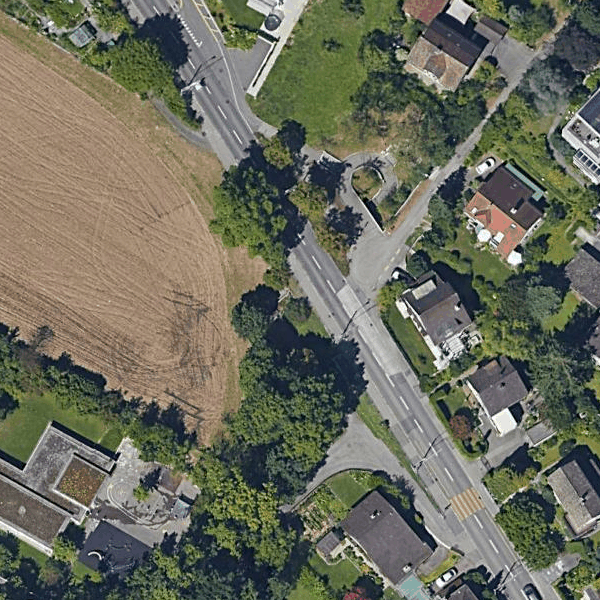
\includegraphics[width=\figfig\textwidth]{1-00-0.png}
	}
	\subbottom[an area of Chicago\label{fig:egchicago}]{
		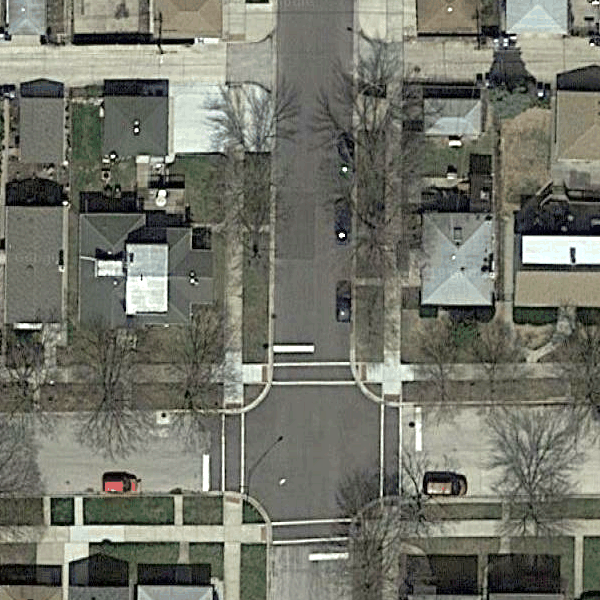
\includegraphics[width=\figfig\textwidth]{1-00-1.png}
	}
    \caption[Example of two satellite images]{Example of two satellite images.}
	\label{fig:egsatimg}
\end{figure}

Nowadays, huge volumes of aerial images are captured with airborne or spaceborne platforms. The increasing volume makes manual interpretation prohibitive \cite{mspascal}. Hence, we should employ appropriate ideas and methods from the field of computer vision to utilize this kind of data. In fact, in order for the machine to better understand aerial images, we can perform image segmentation.

\subsection{Image Segmentation}\label{imgseg}
In the field of computer vision, image segmentation is the process of partitioning an image into multiple sets of pixels. The goal of segmentation is to simplify and change the representation of an image and make the image more meaningful and easier to analyze \cite{cvbookstockman}.

In our project, image segmentation mainly refers to the so-called semantic segmentation, which is a process of labelling each pixel of the image. Hence the segmentation is exactly a pixel-wise classification problem. Note that the labels between two adjacent pixels are not independent, but related to each other. Pixels with the same label are generally similar in the metric of certain visual characteristics, such as color, brightness or texture.

Another kind of segmentation is the so-called instance segmentation. It not only does semantic segmentation, but also distinguishes between the object instances, even they have the same label. That is to say, object instances with same labels are required to have different IDs. Figure \ref{fig:chseg} shows the difference between semantic and instance segmentation.

\begin{figure}[!h]
	\centering
	\subbottom[original image\label{fig:chbfrseg}]{
		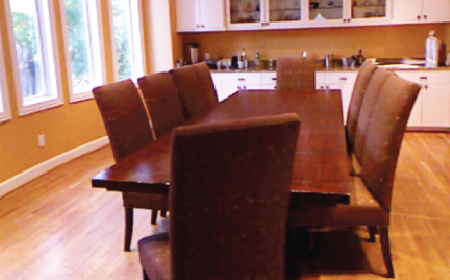
\includegraphics[width=\figfigfig\textwidth]{1-02-0.png}
	}
	\subbottom[semantic segmentation\label{fig:chsemseg}]{
		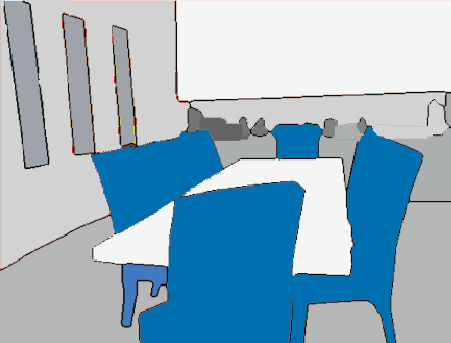
\includegraphics[width=\figfigfig\textwidth]{1-02-1.png}
	}
	\subbottom[instance segmentation\label{fig:chinsseg}]{
		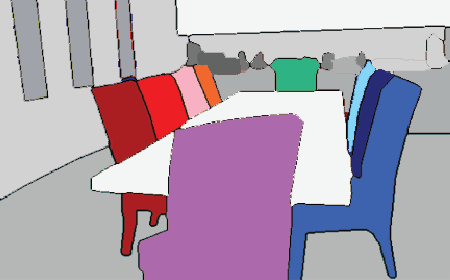
\includegraphics[width=\figfigfig\textwidth]{1-02-2.png}
	}
    \caption[Examples of semantic and instance segmentation]{Examples of semantic segmentation and instance segmentation. Image copyright owned by \cite{chaireccv}. The original image (a) shows a room with several chairs. (b) is the semantic segmentation result of (a), where blue color denotes the chairs, and other colors such as white and gray denote irrelevant background. (c) is instance segmentation result of (a), where all chairs have the same label, but different colors which are used to indicate different instances.}
	\label{fig:chseg}
\end{figure}

Specifically, for semantic segmentation in aerial images, usually what we do is to label each pixel as buildings, roads or background, which can be seen in figure \ref{fig:arsemseg}. Its instance segmentation result is shown in figure \ref{fig:arinsseg}.

\begin{figure}[!h]
	\centering
	\subbottom[original image\label{fig:egbfrseg}]{
		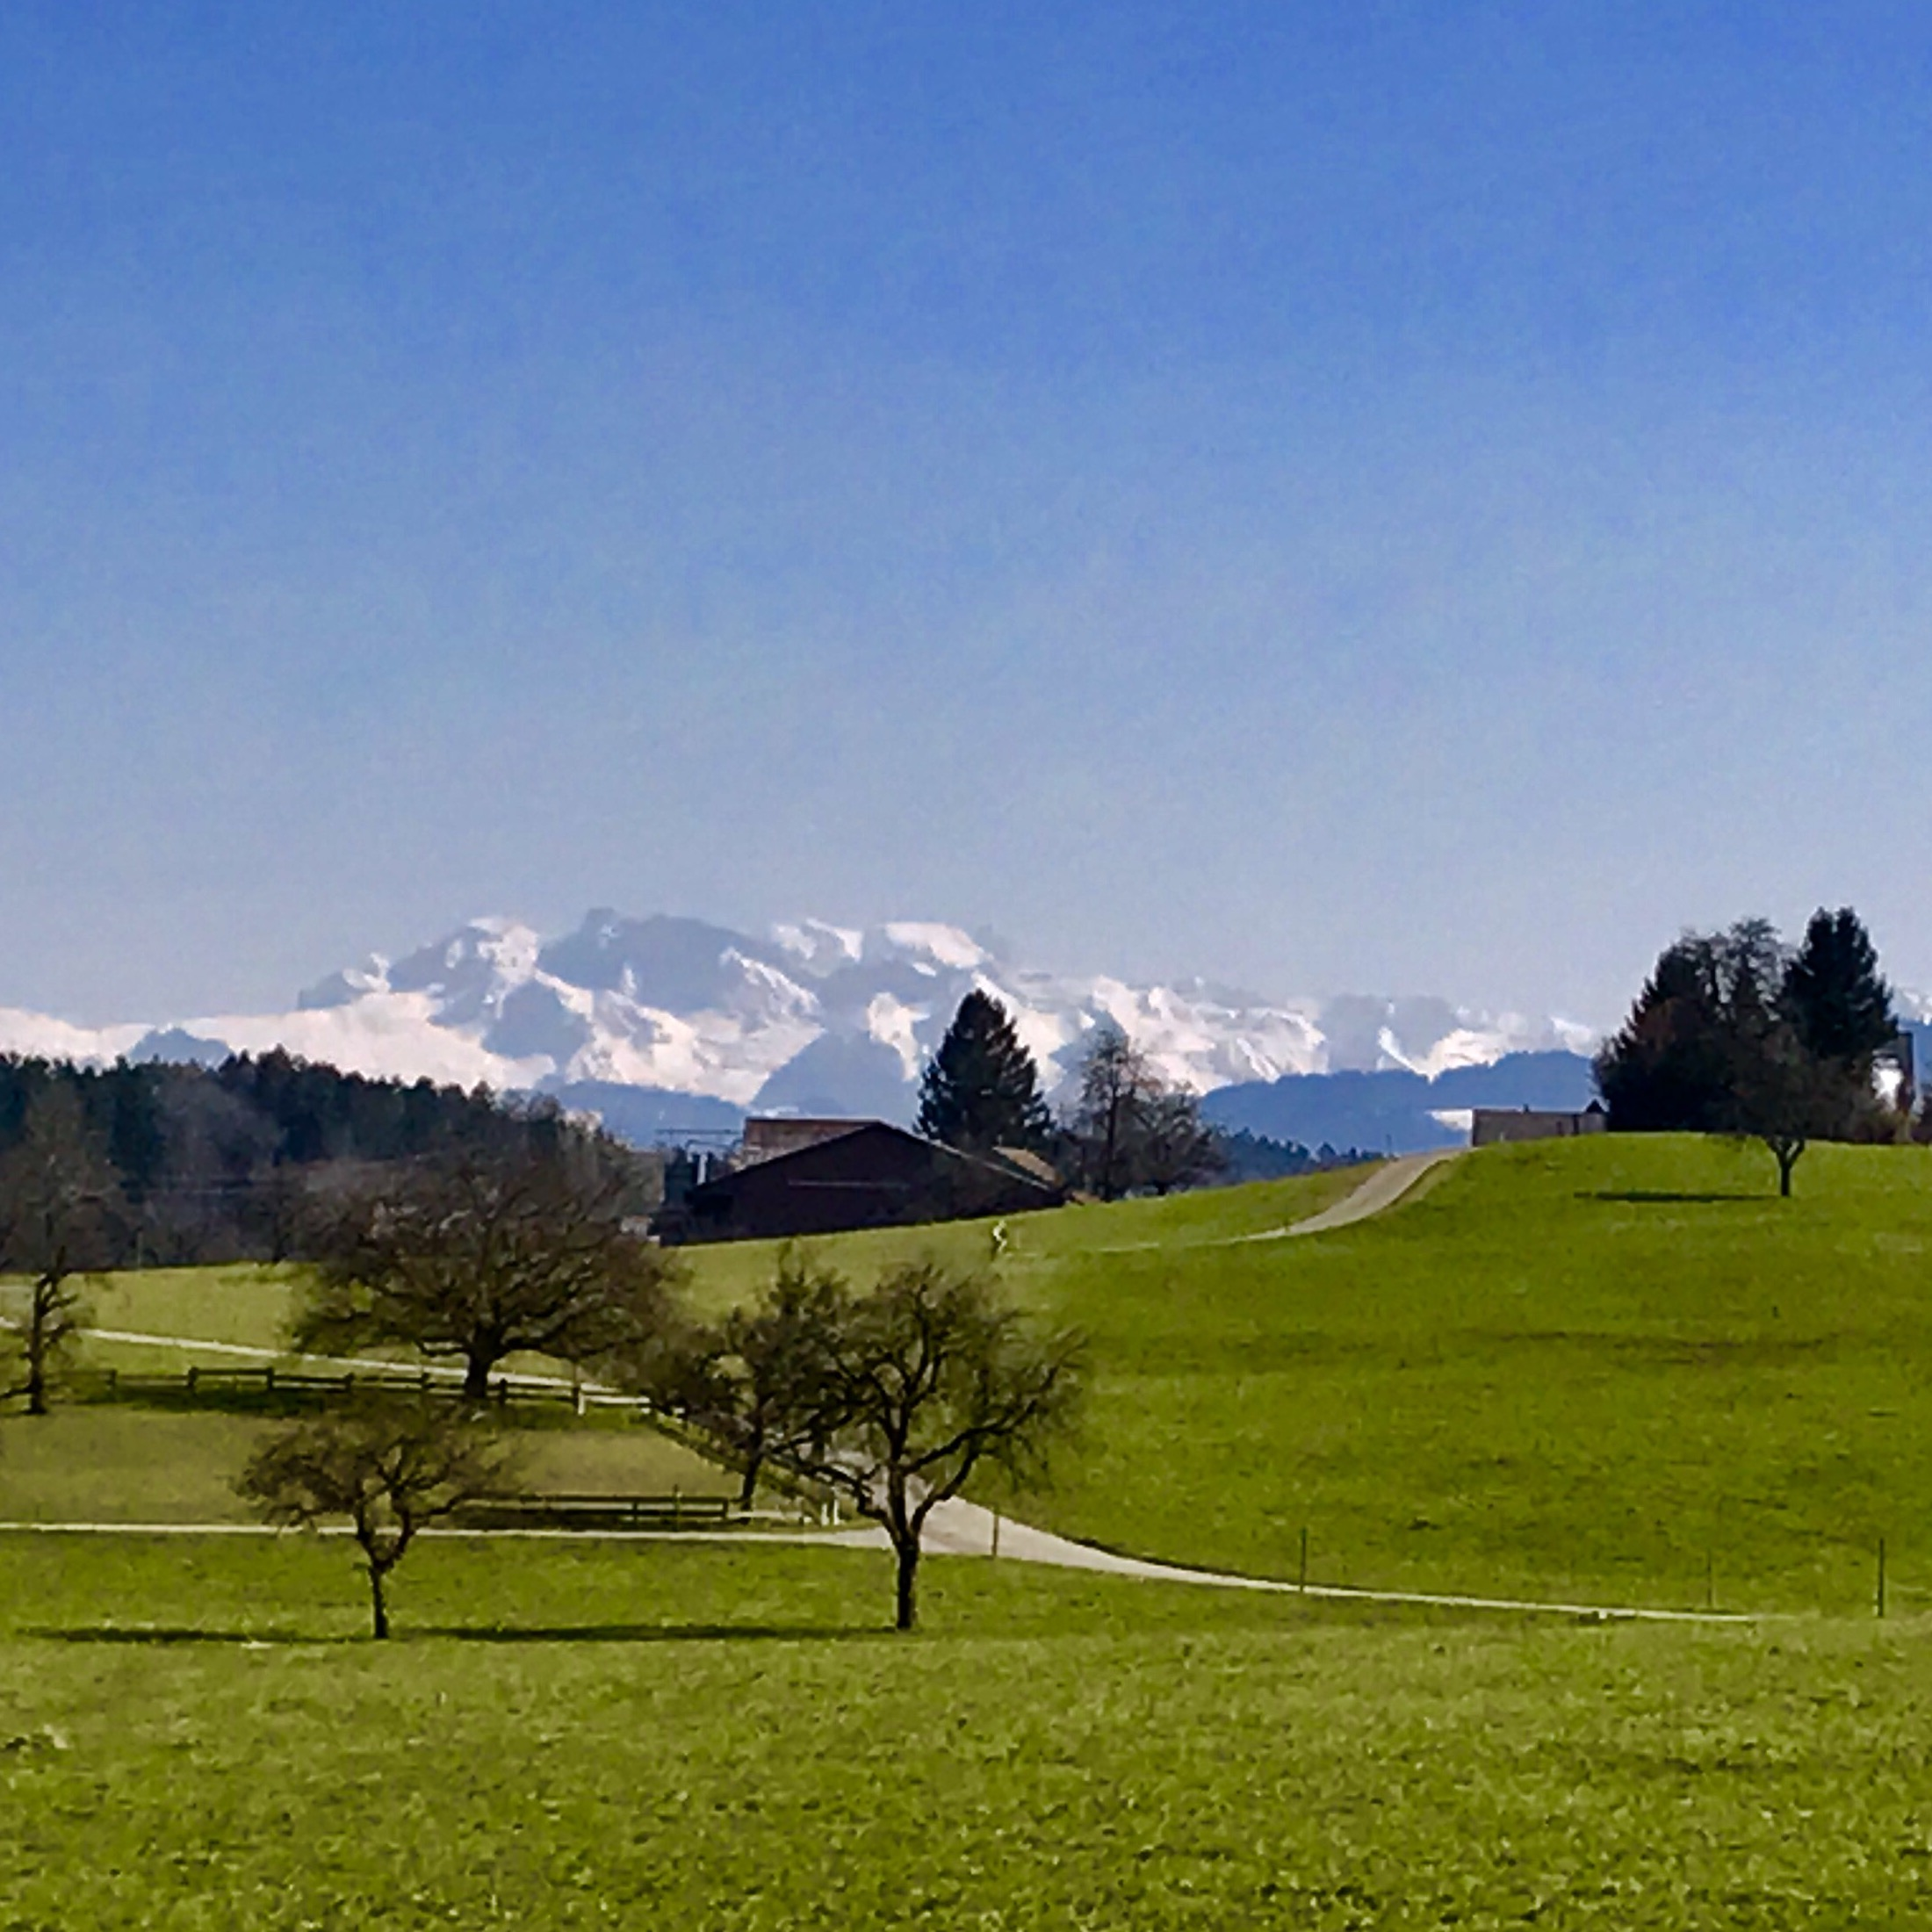
\includegraphics[width=\figfig\textwidth]{1-01-0.jpg}
	}
	\subbottom[image after segmentation\label{fig:egaftseg}]{
		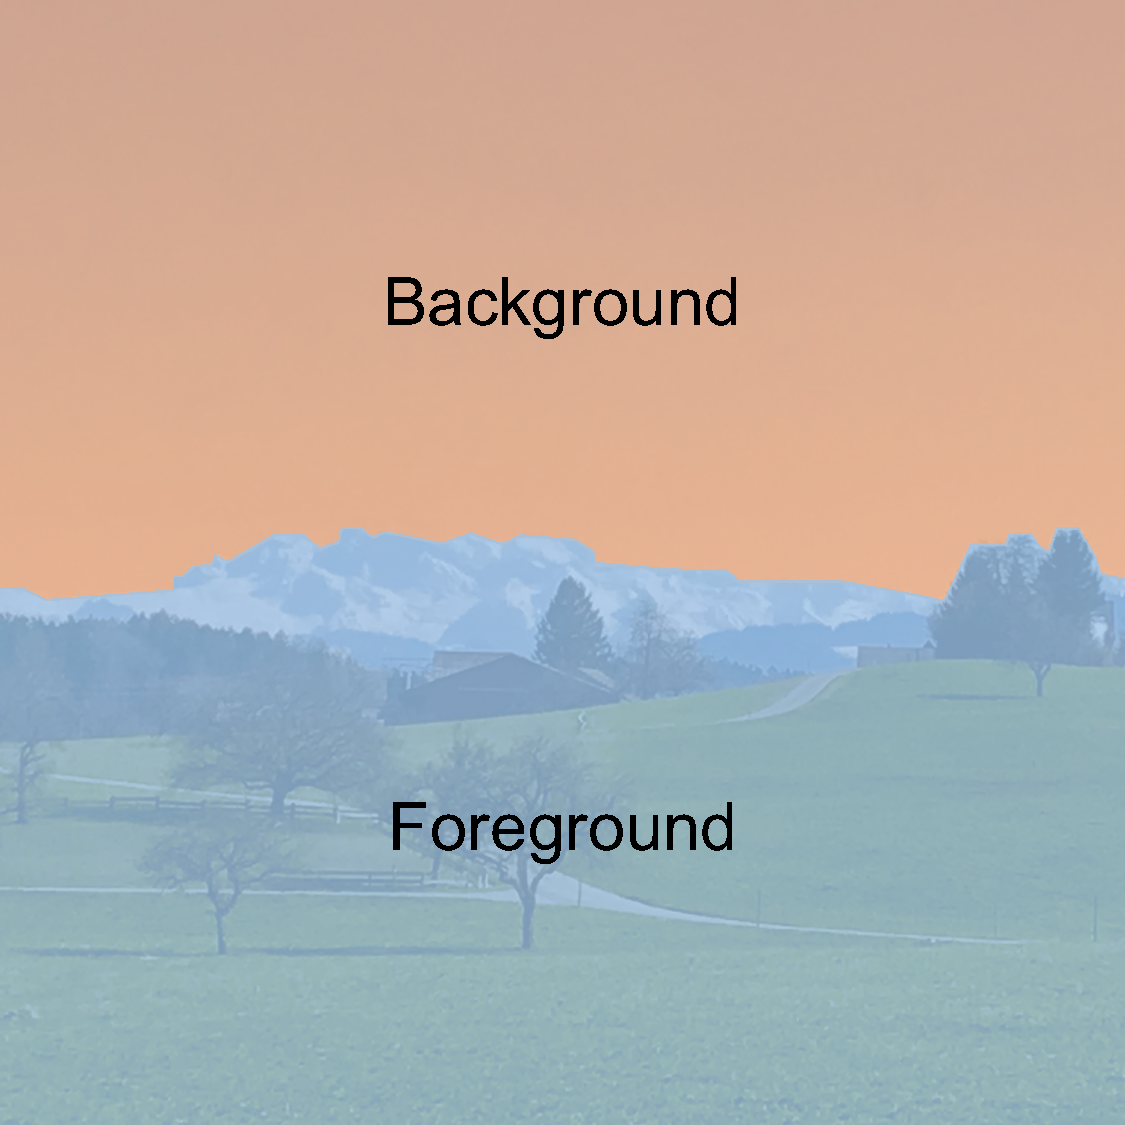
\includegraphics[width=\figfig\textwidth]{1-01-1.pdf}
	}
    \caption[Example of binary image segmentation]{Example of image binary segmentation. The original image (a) is taken from Uetzgi Takeoff.}
	\label{fig:eg01imgseg}
\end{figure}

As a matter of fact, for image where the objects (buildings) are separated like figure \ref{fig:arbfrseg}, we can easily obtain the instance segmentation result based on the pixel connectivity information from the semantic segmentation result. However, if objects overlap in the image like the chairs in figure \ref{fig:chbfrseg}, it is difficult to do such a thing. Thus, in this case, instance segmentation can show its advantages.

Traditional semantic segmentation methods include clustering method \cite{imgsegclustering}, histogram-based method \cite{cvbookstockman}, compression-based methods \cite{imgsegcompress}, region-growing method \cite{imgsegregion} and so on. Recently, deep learning methods have demonstrated remarkable achievements in image segmentation tasks. For those methods, please refer to section \ref{dlimgseg} for more details.

\subsection{Geometrical Shape}\label{geosha}
As introduced in subsection \ref{imgseg}, the output format of either semantic or instance segmentation, is per-pixel mask. Although it is currently the mainstream choice of image segmentation, it is undeniable that the per-pixel mask has limitations on the representation of geometrical shapes. The geometrical shape here generally refers to a polygon represented by a series of ordered vectors or coordinates.

Indeed, we can undergo more processing steps to obtain geometrical shapes based on the instance segmentation result. However, we want to get rid of the pixel-wise labelling rigidity and directly describe geometrical shape of each object in an image. Specifically, in our project, deviating from the standard paradigm of labeling pixels and aiming to directly learn the geometry of the buildings in aerial images have following advantages: (1) Polygon representation has much less redundancy and relatively less storage than pixel-wise labelling; (2) Polygon representation is a kind of vector illustration, thus can be used at arbitrary levels or scales; (3) Buildings with polygon representation can be modeled more naturally; (4) Polygon representation can be directly marked in the electronic map, but per-pixel mask can not. The polygon representation is therefore a more compact, useful and structure-aware representation of object silhouettes in segmentation of buildings on aerial images.

As mentioned in subsection \ref{imgseg}, deep learning methods have shown significant progress in tasks of image segmentation. However, the architectures used in these methods are still limited to conventional grid structure diagrams and their output is still pixel-wise. The rigidity of these networks makes it difficult to exploit high-level priors about the geometrical shapes of objects in the image. 

Therefore, the purpose of this project is to develop novel deep learning methods for the geometrical shapes of arbitrary structures, which means that we want to introduce object geometrical shapes into deep learning techniques.

\section{Problem Definition}\label{prodef}
Given an aerial image, our goal is to extract the polygon shape for each building in the image. The input is an aerial image, denoting 
\begin{equation}
I = \{I_{ijk}\}_{i \in \{1,2,\ldots,h\}, j \in \{1,2,\ldots,w\}, k \in \{1,2,3\}},
\end{equation}
where $I_{ijk}$ denotes the pixel value of $i$-th row, $j$-th column and $k$-th channel in the image, $w$ and $h$ denote the width and height of the input image. The output is polygons, denoting
\begin{equation}
P = \{P^{(n)}\}_{n \in \{1,2,\ldots,N\}},
\end{equation}
\begin{equation}
P^{(n)} = \{(i^{(n)}_t, j^{(n)}_t)\}_{t \in \{1,2,\ldots,L_n\}},
\end{equation}
where $N$ denotes the number of complete buildings (or polygons) in the image, $P^{(n)}$ and $L_n$ denote the $n$-th polygon and its number of vertices, $(i^{(n)}_t, j^{(n)}_t)$ denote the image coordinates of $t$-th vertex of the polygon $P^{(n)}$ in the original input image.

In short, our goal is to achieve instance segmentation of geometrical shapes for buildings in aerial images. Figure \ref{fig:defgeoseg} shows an example of desired input and output.

\begin{figure}[!h]
	\centering
	\subbottom[aerial image as input\label{fig:defgeoseg1}]{
		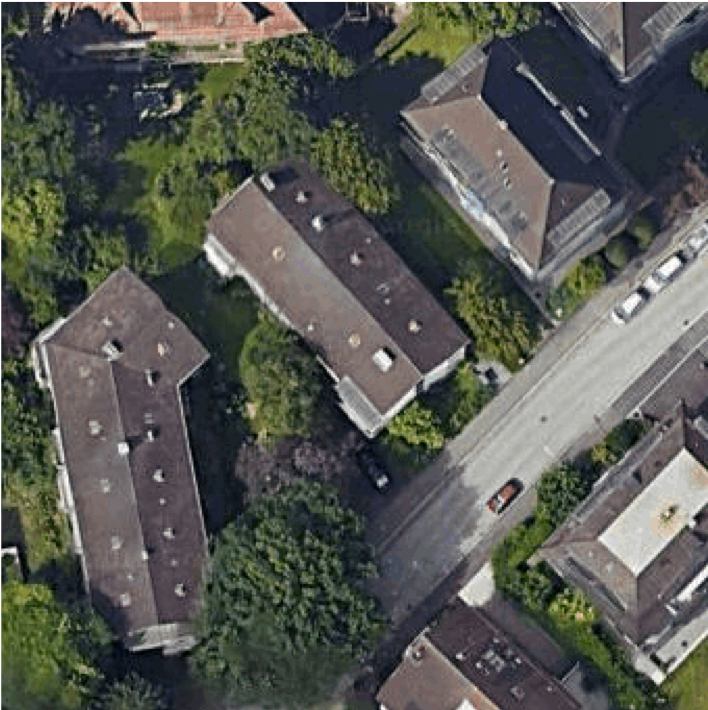
\includegraphics[width=\figfigfig\textwidth]{1-03-0.png}
	}
	\subbottom[expected polygons as output\label{fig:defgeoseg2}]{
		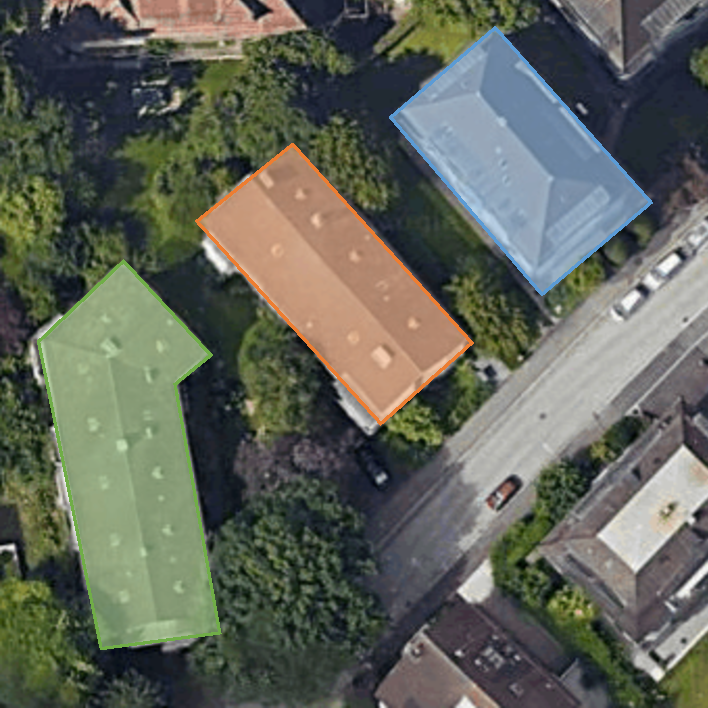
\includegraphics[width=\figfigfig\textwidth]{1-03-1.pdf}
	}
    \caption[Example of instance segmentation of geometrical shapes in an aerial image]{Example of instance segmentation of geometrical shapes in an aerial image. (a) is the input aerial image containing 3 complete buildings. (b) is the visualized result for output polygons.}
	\label{fig:defgeoseg}
\end{figure}

\section{Focus of This Work}\label{fcswrk}
The problem defined in section \ref{prodef} is challenging because it not only requires the correct detection (or localization) for all buildings in an aerial image, but also needs to precisely segmenting each building in the representation of polygon rather than per-pixel mask. Therefore, it is exactly a combination of two tasks of computer vision. The first one is object detection, where the goal is to detect (or localize) each individual object in the image using a bounding box. The second one is the geometrical instance segmentation, where the goal is to extract polygon for a single instance.

In order to solve this problem, we propose a new model, \modelnameshort\ (\modelnamelong), which is a combination of the FPN (Feature Pyramid Network) \cite{fpn} and PolygonRNN \cite{polygonrnn}. In our new model, FPN is used to localize buildings, i.e. to detect the RoIs (Regions of Interest) in the image, and PolygonRNN is used to find geometrical shape for a single object. Experiments show that the new proposed model can successfully find geometrical shapes for multiple buildings in an aerial image.

In summary, our contributions are as follows:
\begin{itemize}
	\item We combine FPN \cite{fpn} and PolygonRNN \cite{polygonrnn}, and propose the model \modelnameshort, with 3 versions. The proposed model tackles the shortcoming of PolygonRNN, which can only segment single object;
	\item We redesign the lateral connection of FPN with VGG-16 \cite{vgg16} backbone in order for the better combination with PolygonRNN;
	\item We learn the idea from \lstinline{seq2seq} \cite{seq2seq} and introduce the beam search algorithm to the prediction phase of PolygonRNN, which addresses the false vertex problem and significantly improves the prediction result.
\end{itemize}

\section{Thesis Organization}\label{thsorg}
This thesis is organized as follows. Chapter \ref{rltwrk} reviews related work, focusing on the deep learning methods for image segmentation, previous work related to segmentation in aerial images, as well as the two recent new models, Mask R-CNN \cite{maskrcnn} and PolygonRNN. In chapter \ref{mdlarc}, the architectures of PolygonRNN and FPN are presented, and the structure of our proposed model is also explained in detail. Chapter \ref{exres} describes the ground truth dataset we use and gives the experiment configurations and results. Finally, chapter \ref{prbftr} makes conclusions, points out the problems which exist in our project and gives future direction.

In addition, the common terminologies used in our project and its corresponding detailed explanations are shown as follows:
\begin{itemize}
	\item \textbf{Object Detection (Object Localization)}:\\
	Detection or localization via bounding boxes instead of masks;
	\item \textbf{Semantic Segmentation}:\\
	Pixel-wise classification without differentiating instances;
	\item \textbf{Instance Segmentation (Semantic Instance Segmentation)}:\\
	Both semantic and a form of detection;
	\item \textbf{Segmentation of Geometrical Shape (Geometrical Segmentation)}:\\
	Extraction of the polygon outlining \textbf{single} object;
	\item \textbf{Instance Segmentation of Geometrical Shapes \\ (Geometrical Instance Segmentation)}:\\
	Both geometrical and a form of detection.
\end{itemize}

